\documentclass{standalone}
\usepackage{chez}

\begin{document}
%\chapter{October 31, 2019}

\subsection{SAT is NP-Complete}
\begin{theorem}[Cook-Levin]
  \(\mathit{SAT}\) is \(\mathsf{NP}\)-complete.
\end{theorem}
\begin{proof}
  We already know that \(\mathit{SAT} \in \mathsf{NP}\).

  Let \(A \in \mathsf{NP}\). We want to show that \(A \polyredu \mathit{SAT}\). In particular, we want to find a reduction \(f \colon w \mapsto \phi_w\) such that \(w \in A \iff \phi_w \in \mathit{SAT}\).

  Let \(A\) be decided by an \textsf{NTM} \(M\) in \(O(n^k)\) time. The key idea is that we will try to make \(\phi_w\) be the statement ``\(M\) accepts \(w\)''.

  \begin{definition*}
    A \vocab{tableau} for \(M\) on \(w\) is an \(N \times N\) table where row \(i\) is the configuration on the \(i\)th step of an accepting branch of \(M\) on \(w\), where the whole branch is \(N\) steps.
    \[
      \begin{array}{| c | c | c | c | c | c | c | c |} \hline % chktex 44
        q_0 & w_1 & w_2 & \!\dots\! & w_n & \blank & \blank & \blank \\ \hline % chktex 44
          &   &   &   &   &   &   &   \\ \hline % chktex 44
          &   &   &   &   &   &   &   \\ \hline % chktex 44
          &   &   &   &   &   &   &   \\ \hline % chktex 44
          &   &   &   &   &   &   &   \\ \hline % chktex 44
          &   &   &   &   &   &   &   \\ \hline % chktex 44
          &   &   &   &   &   &   &   \\ \hline % chktex 44
          &   &   &   &   &   &   &   \\ \hline % chktex 44
      \end{array}
    \]
  \end{definition*}

  We can then think of the statement ``\(M\) accepts \(w\)'' as the statement ``a tableau for \(M\) on \(w\) exists''.

  In particular, we can build \(\phi_w\) with the indicator variables
  \[
    \set*{
      x_{ij\sigma} = \begin{cases}
        1 & \text{cell $(i, j)$ contains $\sigma$} \\[-1ex]
        0 & \text{else},
      \end{cases}
      \mid
      i, j \in \set{1, \dots, N}^2, \sigma \in \tilde\Gamma = \Gamma \union Q
    }.
  \]

  Our formula will be of the form
  \[
    \phi_w = \phi_{\text{cell}} \land \phi_{\text{start}} \land \phi_{\text{move}} \land \phi_{\text{accept}},
  \]
  where
  \begin{itemize}
    \item \(\phi_{\text{cell}}\) checks that each cell has exactly one symbol,
    \item \(\phi_{\text{start}}\) checks that we have the right starting configuration,
    \item \(\phi_{\text{move}}\) checks that each move is valid, and
    \item \(\phi_{\text{accept}}\) checks that the final state is accepting.
  \end{itemize}

  We can write
  \[
    \phi_{\text{cell}} = \bigand_{1 \leq i, j \leq N} \brackets*{
      \bigor_{\sigma \in \tilde\Gamma} x_{ij\sigma} \land
      \bigand_{\substack{\sigma, \tau \in \tilde\Gamma \\ \sigma \neq \tau}} (\ol{x_{ij\sigma}} \lor \ol{x_{ij\tau}})
    }.
  \]
  The outer \(\bigand\) goes through each cell. In particular, the first part inside the bracket says that there must be at least one symbol in each cell, and the second part says that for every pair of symbols \((\sigma, \tau)\), they cannot both be in the cell.

  We have
  \[
    \phi_{\text{start}} = x_{1, k, w} \land \bigand_{k = 1}^{n} x_{1, k + 1, w_k} \land \bigand_{k = n + 1}^{N - 1} x_{1, k, \blank}.
  \]
  This just requires the first row to be \(q_0 w_1 w_2 \dots w_n \blank \dots\). Similarly,
  \[
    \phi_{\text{accept}} = \bigor_{1 \leq i, j \leq N} x_{i, j, q_{\textsc{accept}}}.
  \]

  The hardest subformula to come up with is \(\phi_{\text{move}}\). The idea is that we check that every \(2 \times 3\) subgrid and make sure that the subgrid is valid. In particular, we have
  \begin{align*}
    \phi_{\text{move}}
      &= \bigand_{1 \leq i, j \leq N} [\text{subgrid at $(i, j)$ is valid}] \\
      &= \bigand_{1 \leq i, j \leq N} \brackets*{
          \bigor_{\text{valid $\brackets*{\substack{abc\\def}}$}}
          x_{i, j, a} \land x_{i+1, j, b} \land
          x_{i, j+1, c} \land x_{i+1, j+1, d} \land
          x_{i, j+2, e} \land x_{i+1, j+2, f}
        }.
  \end{align*}
  If \(\phi_{\text{move}}\) is true, 
  Therefore, \(\phi_w\) is an instance of \(\mathit{SAT}\), and a satisfying assignment exists 
\end{proof}

\subsection{Vertex Cover}
Suppose we have an undirected graph \(G = (V, E)\). A \vocab{vertex cover} of \(G\) is a set \(X \subseteq V\) such that every edge \(e \in E\) has at least one end point in \(X\). A \vocab{\(k\)-vertex cover} is a vertex cover of size \(k\).
\begin{example}[Vertex cover]
  The green nodes of the following graph form a \(3\)-vertex cover:
  \begin{center}
    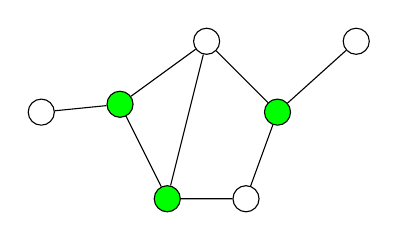
\begin{tikzpicture}[every node/.style={circle, draw}]
      \draw node[fill=green] (a) at (0, 0.2) {};
      \draw node (b) at (-1, 0.1) {};
      \draw node (e) at (1.1, 1) {};
      \draw node[fill=green] (c) at (0.6, -1) {};
      \draw node[fill=green] (f) at (2, 0.1) {};
      \draw node (g) at (3, 1) {};
      \draw node (d) at (1.6, -1) {};

      \draw (a) -- (b)
        (a) -- (c)
        (a) -- (e)
        (c) -- (d)
        (d) -- (f)
        (e) -- (f)
        (f) -- (g)
        (c) -- (e);
    \end{tikzpicture}
  \end{center}
\end{example}

It is natural to then ask the question: given a graph \(G\), does it have a \(k\)-vertex cover? In fact, we define
\[
  \textit{VERTEX-COVER} = \set{\angles{G, k} \mid \text{graph $G$ has a $k$-vertex cover}}.
\]

\begin{proposition}
  \textit{VERTEX-COVER} is \(\mathsf{NP}\)-complete.
\end{proposition}
\begin{proof}
  We will show that \(\textit{3-SAT} \polyredu \textit{VERTEX-COVER}\). Suppose we have an instance \(\phi\) of \textit{3-SAT} with variables \(x_1, \dots, x_k\), and clauses \(c_1, \dots, c_n\), where the clause \(c_i\) contains the literals \(c_i = \ell_{i1} \lor \ell_{i2} \lor \ell_{i3}\). Then consider the graph \(G\) with the following nodes:
  \begin{center}
    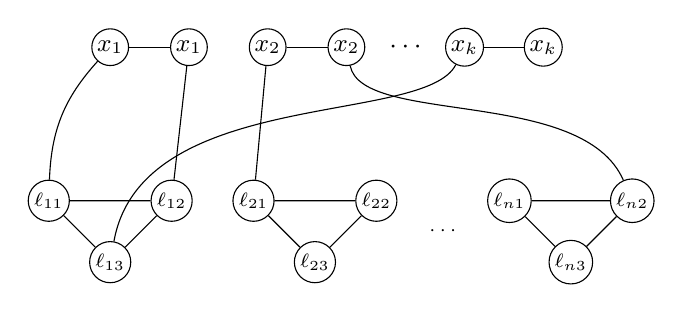
\begin{tikzpicture}
      \begin{scope}[every node/.style={circle, draw, inner sep=1pt, font=\small}]
        \node (x1) at (0, 0) {\(x_1\)};
        \node (X1) at (1, 0) {\(\ol{x_1}\)};
        \node (x2) at (2, 0) {\(x_2\)};
        \node (X2) at (3, 0) {\(\ol{x_2}\)};
        \node (xk) at (4.5, 0) {\(x_k\)};
        \node (Xk) at (5.5, 0) {\(\ol{x_k}\)};

        \begin{scope}[scale=1.3, shift={(-0.6, -1.5)}, every node/.append style={font=\scriptsize}]
          \node (ell11) at (0, 0) {\(\ell_{11}\)};
          \node (ell12) at (1.2, 0) {\(\ell_{12}\)};
          \node (ell13) at (0.6, -0.6) {\(\ell_{13}\)};

          \node (ell21) at (2, 0) {\(\ell_{21}\)};
          \node (ell22) at (3.2, 0) {\(\ell_{22}\)};
          \node (ell23) at (2.6, -0.6) {\(\ell_{23}\)};

          \node (elln1) at (4.5, 0) {\(\ell_{n1}\)};
          \node (elln2) at (5.7, 0) {\(\ell_{n2}\)};
          \node (elln3) at (5.1, -0.6) {\(\ell_{n3}\)};

          \node[draw=none] () at (3.85, -0.3) {\(\cdots\)};
        \end{scope}
      \end{scope}
      \node () at (3.75, 0) {\(\cdots\)};

      \draw (x1) -- (X1)
        (x2) -- (X2)
        (xk) -- (Xk);
      \draw (ell11) -- (ell12) -- (ell13) -- (ell11);
      \draw (ell21) -- (ell22) -- (ell23) -- (ell21);
      \draw (elln1) -- (elln2) -- (elln3) -- (elln1);

      \draw (x1) to[bend right=20] (ell11);
      \draw (X1) to (ell12);
      \draw (xk) .. controls (4, -1) and (0.4, -0.5) .. (ell13);

      \draw (x2) to (ell21);
      \draw (X2) .. controls (3.2, -1) and (6, -0.5) .. (elln2);
    \end{tikzpicture}
  \end{center}
  We have two connected nodes for each variable \(x_i\). One for \(x_i\) and one for \(\ol{x_i}\). We also have three connected nodes for each clause, one for each literal. Then, we also connect the variable nodes with the corresponding literals if they are the same. We then consider the reduction
  \[
    f \colon \angles{\phi} \mapsto \angles{G, k + 2n}.
  \]
  Note that to cover the edges between the variables \(x_i\) and \(\ol{x_i}\), we need to use at least \(k\) vertices on the top. Similarly, to get all of the edges for the clauses, we need to use at least \(2n\) vertices on the bottom. Therefore, it must be this distribution.

  If \(\phi\) has a satisfying assignment, then there exists some assignment for each \(x_i\). This corresponds to the \(k\) vertices we select on top. Then, since all of the clauses are satisfied, for each clause \(c_i\) there exist some literal \(\ell_{ij}\) in the clause that is satisfied. In particular, the edge from the variable to the literal is covered by the variable. Therefore, the \(2\) nodes we select for the clause can be the other \(\ell_{ij'}\), and all edges relevant to that clause will be covered.

  Similarly, if \(G\) has a \((k + 2n)\)-vertex cover, then there is a set with \(k\) vertices on the top and \(2n\) on the bottom. The \(k\) vertices correspond to the assignment of variables. Then for each clause \(c_i\), we can only select \(2\) of the \(3\) vertices \(\set{\ell_{i1}, \ell_{i2}, \ell_{i3}}\). This means that the edge connecting the last literal edge must be covered with the variable vertex, implying that the clause is satisfied.
\end{proof}

% todo do the n by n triangle thing for A_CFG in P proof

\subsection{ALLCUT Problem}
Consider a set of vertices \(V\). Let \(T\) be a set of subsets of \(V\) with size \(3\). We can think of these as like `edges', but they have three nodes. % thredges
Suppose we color each node either blue or red. Call an triple \(t \in T\) \vocab{happy} if it has at least one blue node and one red node. Then we can define the problem
\[
  \textit{ALLCUT} = \set{
    \angles{V, T} \mid \text{$V$ is a set of nodes with triples $T$ that can be colored such that all triples are happy}
  }.
\]

\begin{example}
  All of the triples of the following graph with its coloring are happy:
  \begin{center}
    \begin{tikzpicture}[
      every node/.style={circle, draw},
      bnode/.style={blue, fill={cyan!10!white}},
      rnode/.style={red, fill={red!10!white}},
      shorten <=2pt,
    ]
      \draw node[bnode] (v1) {};
      \draw node[rnode, below right=0.3 and 1.2 of v1] (v2) {};
      \draw node[rnode, below right=1.2 and 0.0 of v1] (v3) {};
      \draw node[bnode, below right=1.1 and 0.6 of v2] (v4) {};
      \draw node[bnode, above right=0.7 and 1.2 of v2] (v5) {};
      \draw node[rnode, below right=0.0 and 1.2 of v5] (v6) {};
      \draw node[rnode, below right=1.3 and 0.3 of v5] (v7) {};
      \draw node[bnode, below right=0.2 and 1.2 of v7] (v8) {};

      \coordinate[at=($(v1)!0.5!(v2)!0.33!(v3)$)] (e1);
      \coordinate[at=($(v2)!0.5!(v4)$)] (e2);
      \coordinate[at=($(v2)!0.5!(v5)$)] (e3);
      \coordinate[at=($(v5)!0.5!(v6)!0.4!(v7)$)] (e4);
      \coordinate[at=($(v7)!0.5!(v8)$)] (e5);

      \draw (v1) -- (e1);
      \draw (v2) -- (e1);
      \draw (v3) -- (e1);
      \draw (v2) -- (e2);
      \draw (v4) to[bend left] (e2);
      \draw (v4) to[bend right] (e2);
      \draw (v2) -- (e3);
      \draw (v5) to[bend left] (e3);
      \draw (v5) to[bend right] (e3);
      \draw (v5) -- (e4);
      \draw (v6) -- (e4);
      \draw (v7) -- (e4);
      \draw (v7) -- (e5);
      \draw (v8) to[bend left] (e5);
      \draw (v8) to[bend right] (e5);
    \end{tikzpicture}
  \end{center}

  In contrast, the following vertices with triples shown do not have a coloring that makes all triples happy:
  \begin{center}
    \begin{tikzpicture}[
      every node/.style={circle, draw},
      bnode/.style={blue, fill={cyan!10!white}},
      rnode/.style={red, fill={red!10!white}},
      shorten <=2pt,
    ]
      \draw node (v1) {};
      \draw node[below right=0.3 and 1.2 of v1] (v2) {};
      \draw node[below right=1.2 and 0.0 of v1] (v3) {};

      \coordinate[at=($(v1)!0.5!(v2)$)] (e1);
      \coordinate[at=($(v2)!0.5!(v3)$)] (e2);
      \coordinate[at=($(v3)!0.5!(v1)$)] (e3);

      \draw (v1) -- (e1);
      \draw (v2) to[bend left] (e1);
      \draw (v2) to[bend right] (e1);
      \draw (v2) -- (e2);
      \draw (v3) to[bend left] (e2);
      \draw (v3) to[bend right] (e2);
      \draw (v3) -- (e3);
      \draw (v1) to[bend left] (e3);
      \draw (v1) to[bend right] (e3);
    \end{tikzpicture}
  \end{center}
\end{example}

\begin{claim}
  \(\textit{ALLCUT}\) is \(\mathsf{NP}\)-complete.
\end{claim}
\begin{proof}
  First, we know that \(\textit{ALLCUT} \in \mathsf{NP}\) because we can nondeterministically guess the color for each vertex. We will show that \(\textit{ALLCUT}\) is \(\mathsf{NP}\)-hard by proving \(\textit{3-SAT} \polyredu \textit{ALLCUT}\).

  The key idea is that since we want to embed an asymmetrical problem in a symmetrical setting, we introduce a way to get rid of the redundancy. In this problem, we're trying to map true formulas to a colored graph, we will have two connected template nodes for the values of \textsc{true} and \textsc{false}. We can force them to have opposite colors by connecting them both with an edge, where one of them is connected twice.
  \begin{center}
    \begin{tikzpicture}[
      every node/.style={circle, draw, inner sep=2pt},
      bnode/.style={blue, fill={cyan!10!white}},
      rnode/.style={red, fill={red!10!white}},
      shorten <=2pt
    ]
      \draw node[bnode] (T) {\footnotesize T};
      \draw node[rnode, right=of T] (F) {\footnotesize F};
      \coordinate[at=($(T)!0.5!(F)$)] (e);
      \draw (T) -- (e);
      \draw (F) to[bend left] (e);
      \draw (F) to[bend right] (e);
    \end{tikzpicture}
  \end{center}
  Then, we can connect other things to these nodes in order to enforce which color means true and which means false.

  In our graph, we will also have a node for each possible literal,
  i.e.\ two nodes for each variable.
  We can force all of these to have opposite colorings
  using the same method we did for \textsc{true} and \textsc{false}.
  \begin{center}
    \begin{tikzpicture}[
      every node/.style={circle, draw, inner sep=2pt},
      bnode/.style={blue, fill={cyan!10!white}},
      rnode/.style={red, fill={red!10!white}},
      shorten <=2pt
    ]
      \draw node[bnode] (T) {\small \(x_i\)};
      \draw node[rnode, right=of T] (F) {\small \(\ol{x_i}\)};
      \coordinate[at=($(T)!0.5!(F)$)] (e);
      \draw (T) -- (e);
      \draw (F) to[bend left] (e);
      \draw (F) to[bend right] (e);
    \end{tikzpicture}
  \end{center}

  Consider some clause \(c = \ell_1 \lor \ell_2 \lor \ell_3\). We want to encode the fact that at least one of the literals is \textsc{true}. To do this, we can form a new node for the clause, and then connecting the following nodes is sufficient:
  \begin{center}
    \begin{tikzpicture}[
      every node/.style={circle, draw, minimum size=0.5cm, inner sep=1pt},
      bnode/.style={blue, fill={cyan!10!white}},
      rnode/.style={red, fill={red!10!white}},
      shorten <=2pt,
    ]
      \node (l1) {\(\ell_1\)};
      \node[below=of l1] (l2) {\(\ell_2\)};
      \node[right=3 of l1] (l3) {\(\ol{\ell_3}\)};
      \node[at=($(l2)!0.5!(l3)$)] (center) {\(c\)};
      \node[bnode, below=of l3] (t) {\footnotesize T};
      
      \coordinate[at=($(l1)!0.5!(l2)!0.4!(center)$)] (e1);
      \coordinate[at=($(l3)!0.5!(t)!0.4!(center)$)] (e2);
      \draw (l1) -- (e1);
      \draw (l2) -- (e1);
      \draw (center) -- (e1);
      \draw (l3) -- (e2);
      \draw (t) -- (e2);
      \draw (center) -- (e2);
    \end{tikzpicture}
  \end{center}
  To see why this works, note that if both \(\ell_1\) and \(\ell_2\) are colored with the same color as \textsc{false}, then the node labeled \(c\) must be colored \textsc{true}. Then, this forces \(\ol{\ell_3}\) to be colored \textsc{false}, which means \(\ell_3\) is true.

  Now, if \(\phi\) is an instance of \textit{3-SAT} that is satisfiable, then we color each node corresponding to each literal with its truth value. Then, it is easy to check that the \(c\) node corresponding to a clause can be colored.

  Conversely, if the graph is colorable, then we can take the colors that we have assigned to the literal clauses and get the assignment of values.
\end{proof}


\subsection{MAXCUT is NP-Complete}
Consider an undirected graph \(G = (V, E)\) and some \(k \in \NN\). Call an edge \vocab{happy} if we can color each node such that each edge has both colors. Let
\[
  \textit{MAXCUT} = \set{
    \angles{G = (V, E), k} \mid \text{$G$ is a graph such that at least $k$ edges are happy}
  }.
\]

\begin{example}
  For the following graph \(G\), we have \(\angles{G, 3} \in \textit{MAXCUT}\) but \(\angles{G, 4} \notin \textit{MAXCUT}\).
  \begin{center}
    \begin{tikzpicture}[
      every node/.style={circle, draw},
      shorten <=1pt, shorten >=1pt,
    ]
      \node (v1) {};
      \node[right=of v1] (v2) {};
      \node[above right=1 and 0.5 of v1] (v3) {};
      \node[right=of v3] (v4) {};

      \draw (v1) -- (v2);
      \draw (v2) -- (v3);
      \draw (v3) -- (v1);
      \draw (v3) -- (v4);
    \end{tikzpicture}
  \end{center}
\end{example}

\begin{claim}
  \(\textit{MAXCUT}\) is \(\mathsf{NP}\)-complete.
\end{claim}
\begin{proof}
  It is clear that \(\textit{MAXCUT} \in \mathsf{NP}\) because we can just nondeterministically guess the coloring.

  To prove that \(\textit{MAXCUT}\) is \(\mathsf{NP}\)-hard, we will show that \(\textit{ALLCUT} \polyredu \textit{MAXCUT}\). Suppose we have an instance \(\angles{V, T}\) of \(\textit{ALLCUT}\). Then, for each triple \(\set{u, v, w} \in T\), we make three edges \(\set{u, v}\), \(\set{v, w}\), and \(\set{w, u}\). If the original triple was happy, then exactly two of the new edges are happy. Therefore, we replace all triples in the original graph with these triangles, and require that \(K = 2 \size{T}\). In particular, \(f(V, T) = \angles{V, 2\size{T}}\).
\end{proof}

% [proving things about N and NP] is like handling hot food with mittens
% you dont know that the food is hot but you still want to move it




\end{document}

